\documentclass{article}
\usepackage[utf8]{inputenc}
\usepackage{graphicx}
\usepackage{amsmath}

\title{15463 Assignment 5}
\author{Lingxi Zhang (lingxiz)}
\date{November 18, 2022}

\begin{document}

\maketitle

\section{Photometric stereo}
\subsection{Uncalibrated photometric stereo}
\begin{figure}[ht]
    \centering
    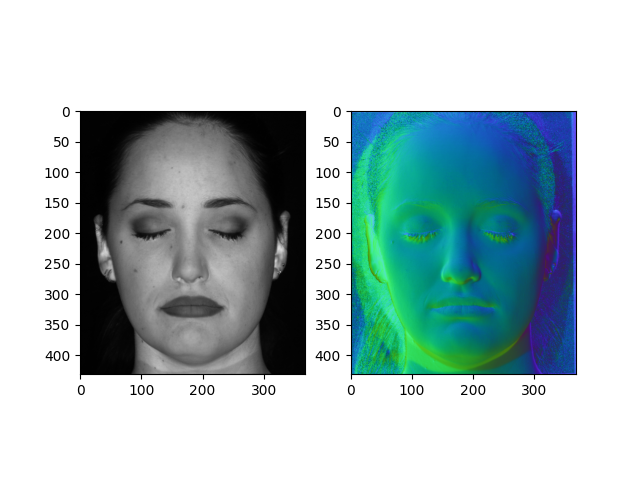
\includegraphics[scale=0.8]{../data/output/default.png}
    \caption{$\mathbf{A_e}$ and $\mathbf{N_e}$}
\end{figure}
\begin{figure}[ht]
    \centering
    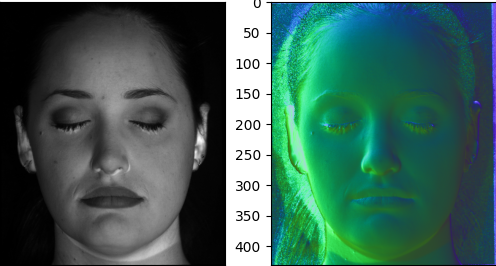
\includegraphics[scale=0.8]{../data/output/Q.png}
    \caption{$\mathbf{A_Q}$ and $\mathbf{N_Q}$}
\end{figure}

where 
\begin{align}
Q =
\begin{bmatrix}
    1 & 0.5 & 0.5\\
    0.25 & 1 & 0.25 \\
    0.5 & 0.5 & 1
\end{bmatrix}
\end{align}

\subsection{Enforcing integrability}


\begin{figure}[ht]
    \centering
    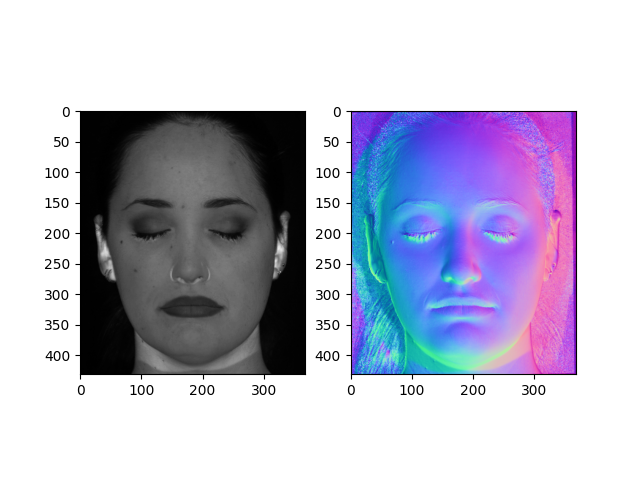
\includegraphics[scale=0.8]{../data/output/enforce.png}
    \caption{$\mathbf{A_Q}$ and $\mathbf{N_Q}$}
\end{figure}
\newpage

\subsection{Normal integration}




\subsection{calibrated photometric stereo}




\section{Capture and reconstruct your own shapes}

\end{document}
